\chapter{3D object representation}

This chapter contains the definitions for various three-dimensional object representations
that are commonly used in applications. A geometric query or a different operation involving the
object might be more effectively formulated with one representation than another.

\section{Overview}

The 3D object representations can be divided into two big categories

\begin{itemize}
\item \textbf{solid} - the object in this representation contains information about inner
propreties of the object such as density or elasticity. It is mostly used in software for
engineering simulations.

\item \textbf{surface} - this representation works only with the surface of the object
ignoring the properties of the volume. The one of advantages of this representation is
relatively simple visualisation. The surface description is totally sufficient for graphical purposes.
\end{itemize}

\subsection{Voxel map}

A \textbf{voxel} is a word made by joining '\textbf{Vo}lumetric' and 'Pi\textbf{xel}'. It represents
the value on regular grid that forms a voxel map. The simpliest representation of voxel map is
normalized grid made of cube-shaped voxels with 0-1 values where 0 stands for that cube is completely
outside of the object and 1 represents the case of crossing the surface or inclusion by the object.
\\
\\
Each voxel can contain various properties such as color, material physical properties or
in case of boundary voxels, surface description. Some implementation provide information about
each corner of voxel separately in order to improve the accuracy.
As can be deduced from overview, this representation perfectly fits for representing the solid objects.

\subsection{Isosurface}

\subsection{Constructive solid geometry}

Known also as \emph{CSG tree}. This technique is used especially in engineering software. It allows
user to construct objects using \emph{Boolean operators} to combine objects. Objects created using this
method can be used repeatedly in Boolean operators; resulting object can be decomposited into a tree.
\\
\\
The leafs of the tree are typically the objects of the simple shape, however the operators can be
theoretically applied on any objects. The set of supported primitives are given by a specific
software package.
\\
\\
Thanks to the tree structure, CSG objects come with some convenient properties. The nodes that
are higher in the tree hierarchy gives us an approximation that can be used in various geometric
algorithms with no need for searching its descendants.

\subsection{Point cloud}

A point cloud is a set of points in three-dimensional coordinate system. The set can form the surface
of an object or any other three dimensional figure. Each point is indepedent
from each other, with no information about its topology. Often they are converted to polygon mesh
or triangle mesh models.

\subsection{Polygonal mesh}

A polygonal mesh is a collection of vertices, edges and faces that defines the shape of the surface of
the object. Some special implementations do not contain faces, those are defined only by vertices and
edges. Moreover, some cases do not consider the topology and the object is a raw set of polygons.
Neverthless, standard implementation is expected to contain a topology information about each vertex
and face.
\\
\\
Each face is defined by planar polygon, in special cases by \emph{convex polygon} or \emph{triagle}.
The polygonal mesh restricted to contain triangular faces only is called \emph{triangle mesh}.
The main purpose of restriction is the rendering simplification. In general case, face is defined
as the set of points that can contain a hole.
\\
\\
There are several techniques to represent a topology of the mesh. Each of them has its own advantages
that are reflected in efficiency of data storage and querying the surrounding elements. Several
mesh representations are described in the next section.

\section{Polygonal Mesh}

The collection can be represented in a variety ways, the main purpose of structure is to improve
the efficiency of the queries. In the other hand we face the limitations such as memory. In some
representations in impossible to query the adjacent vertices of a vertex without iteration through
entire container of vertices or faces.

\subsection{Face-vertex mesh}

The simpliest representation that contains any information about topology of the polygonal
mesh. A mesh is represented by a container of vertices and the container of sets of vertices that
forms faces. The face is represented by at least 3 vertices or more vertices that have to be
coplanar.\\

\begin{figure}[h]

\begin{minipage}[hb]{0.65\linewidth}
\centering
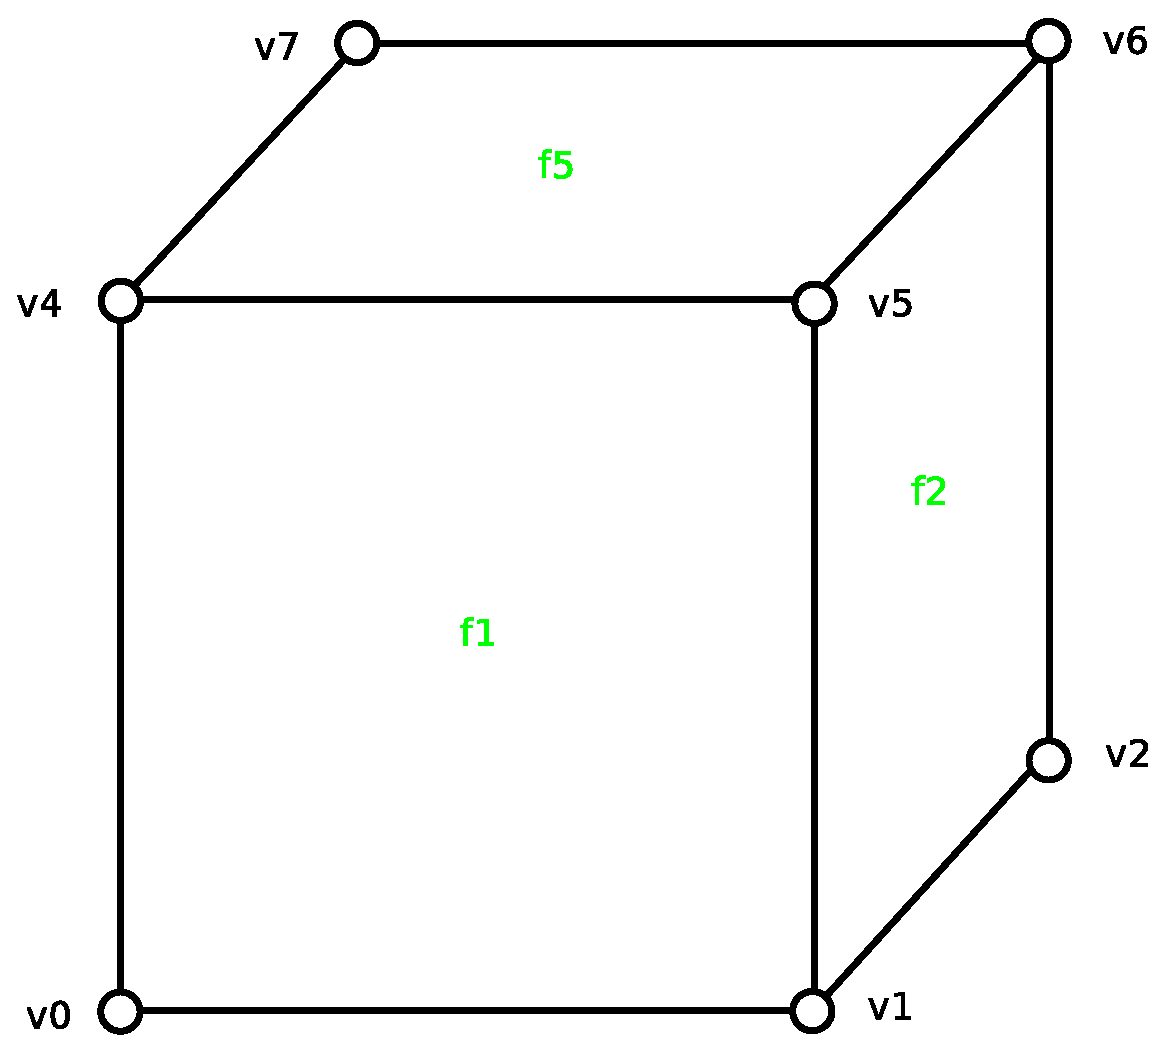
\includegraphics[width=0.6\linewidth]{../img/fv_rep_mesh.eps}
\label{fig:figure1}
\end{minipage}
\hspace{0.5cm}
\begin{minipage}[hb]{0.25\linewidth}
\centering
\begin{tabular}{|c|c|}
\hline
\textsf{v0 v1 v5 v4} & \textsf{f1}\\
\hline
\textsf{v1 v2 v6 v5} & \textsf{f2}\\
\hline
\textsf{v4 v5 v6 v7} & \textsf{f5}\\
\hline
\end{tabular}
\label{fig:figure2}
\end{minipage}

\end{figure}

The set that forms the faces must be ordered. The preceding and following vertex in order must be adjacent to
the vertex. If the structure is not extended by face-normal-attribute, the vertices must be in 
clockwise/counter-clockwise order from the view of face normal. If the order is either clockwise or counter-clockwise
depends on the implementation of the mesh.

\subsection{Winged-edge mesh}

The representation described above contain no direct information about adjacency of faces. 
In order to determine the adjacency of any two faces or vertices in constant complexity, we
can build a structure that requires an extra storage. The winged edge structure provide information
that are capable of determination an edges that belong to a vertex, from a given face a set
of edges that surrounds the face; in case of triangle mesh, it returns the triplet of edges.
Finally, the name \emph{winged-edge} is due to capabilty to get a face pair (wings) from
a given edge.


\subsection{Half-edge mesh}
